{\color{gray}\hrule}
\begin{center}
\section{Method Analysis}
\textbf{Hardware analysis}
\bigskip
\end{center}
{\color{gray}\hrule}

\begin{multicols}{2}
\subsection{Methodology}
Over time, different researchers have utilized various testing environments and hardware configurations to evaluate their energy-aware scheduling algorithms. To examine the evolution of their experimental approaches, we have collected and structured data from the selected papers, focusing on the simulation environment, the number of CPU Cores, memory capacity, and power consumption of the experimentation hardware. Specifically, we define:
\begin{itemize}
    \item \textbf{P idle (W)} as the power consumption at low CPU utilization (generally below 50\% load).
    \item \textbf{P max (W)} as the power consumption at maximum CPU load.
\end{itemize}

In some studies, multiple hardware configurations were reported—either due to hardware availability or to assess performance on more powerful setups. In these cases, multiple entries are provided in the table. Note that when power consumption figures were not experimentally reported but instead obtained from hardware specification (by searching for the make and model), those values are marked with an asterisk (\textasteriskcentered). Whenever certain data fields were omitted by the authors, we use ``Nm'' (not mentioned).

\end{multicols}
\begin{table}[H]
\centering
\footnotesize
\begin{tabular}{|p{3.8cm}|p{2.2cm}|p{1.2cm}|p{1.5cm}|p{1.8cm}|p{1.8cm}|}
\hline
\textbf{Paper Ref.} & \textbf{Simulation Environment} & \textbf{CPU Cores} & \textbf{Memory (GB)} & \textbf{Power P idle (W)} & \textbf{Power P max (W)} \\
\hline
Availability-Aware Scheduler \cite{alahmad_availability-aware_2018} (2018) & CloudSim & Nm & Nm & Nm & Nm \\
\hline
Renewable-Aware Scheduling \cite{kumar_renewable_2019} (2019) & Nm & 4 & 64 & 100 & 150 \\
\hline
Renewable-Aware Scheduling \cite{kumar_renewable_2019} (2019) & Nm & 8 & 128 & 120 & 200 \\
\hline
Renewable-Aware Scheduling \cite{kumar_renewable_2019} (2019) & Nm & 16 & 256 & 150 & 250 \\
\hline
Concurrent Container Scheduling \cite{hu_concurrent_2020} (2020) Homogeneous Cluster & ExoGENI & 2 & 6 & Nm & Nm \\
\hline
Concurrent Container Scheduling \cite{hu_concurrent_2020} (2020) & ExoGENI & 1 & 3 & Nm & Nm \\
\hline
Concurrent Container Scheduling \cite{hu_concurrent_2020} (2020) & ExoGENI & 2 & 6 & Nm & Nm \\
\hline
Concurrent Container Scheduling \cite{hu_concurrent_2020} (2020) & ExoGENI & 4 & 12 & Nm & Nm \\
\hline
GP Hyper-Heuristic for Containers \cite{tan_hybrid_2019} (2019) & Nm & Nm & 0.8 & Nm & Nm \\
\hline
PSO-Based Container Consolidation \cite{shi_energy-aware_2018} (2018) & Nm & 4 & 16 & Nm & Nm \\
\hline
Energy-Efficient Container Framework \cite{piraghaj_framework_2015} & CloudSim & 4 & 64 & 86 & 117 \\
\hline
Energy-Efficient Container Framework \cite{piraghaj_framework_2015} & CloudSim & 8 & 128 & 93 & 135 \\
\hline
Energy-Efficient Container Framework \cite{piraghaj_framework_2015} & CloudSim & 16 & 256 & 66 & 247 \\
\hline
VM Consolidation Strategy \cite{carrega_energy-aware_2017} (2017) & Nm & 2 & Nm & 170 & 220 \\
\hline
Predictive Resource Provisioning \cite{dabbagh_energy-efficient_2015} (2015) & Nm & Nm & Nm & 107 & 300.81 \\
\hline
Dynamic VM Reallocation \cite{beloglazov_energy_2010} (2010) & Nm & 1 & 8 & Nm & Nm \\
\hline
Autonomic Container Management \cite{barna_delivering_2017} (2017) & LEGIS & Nm & 16 & Nm & Nm \\
\hline
Brownout-Based Scheduling \cite{xu_energy_2016} & CloudSim & 2 & 4 & 156\textasteriskcentered & 247\textasteriskcentered \\
\hline
GPR + Convex VM Planning \cite{bui_energy_2017} (2017) & Nm & 4 & 12 & 225\textasteriskcentered & 375\textasteriskcentered \\
\hline
SLA-Aware Consolidation \cite{li_sla-aware_2018} (2018) & CloudSim & 2 & 4 & 102 & 117 \\
\hline
SLA-Aware Consolidation \cite{li_sla-aware_2018} (2018) & CloudSim & 2 & 4 & 116 & 135 \\
\hline
\end{tabular}
\centering
\caption{Hardware and Power Specifications}
\label{tab:hardware_specs}
\end{table}
\begin{multicols}{2}

\subsection{Plots and Visualization}
We visualized the simulation environments used in each paper over time to observe how they have evolved (Figure~\ref{fig:timeline}). Each point corresponds to a paper, placed according to its publication year and the simulation platform it utilized (CloudSim, ExoGENI, LEGIS, or ``Nm'' if not mentioned) Each point denotes a paper, positioned by its publication year and the simulation platform it utilized.. 


\begin{figure}[H]
    \centering
    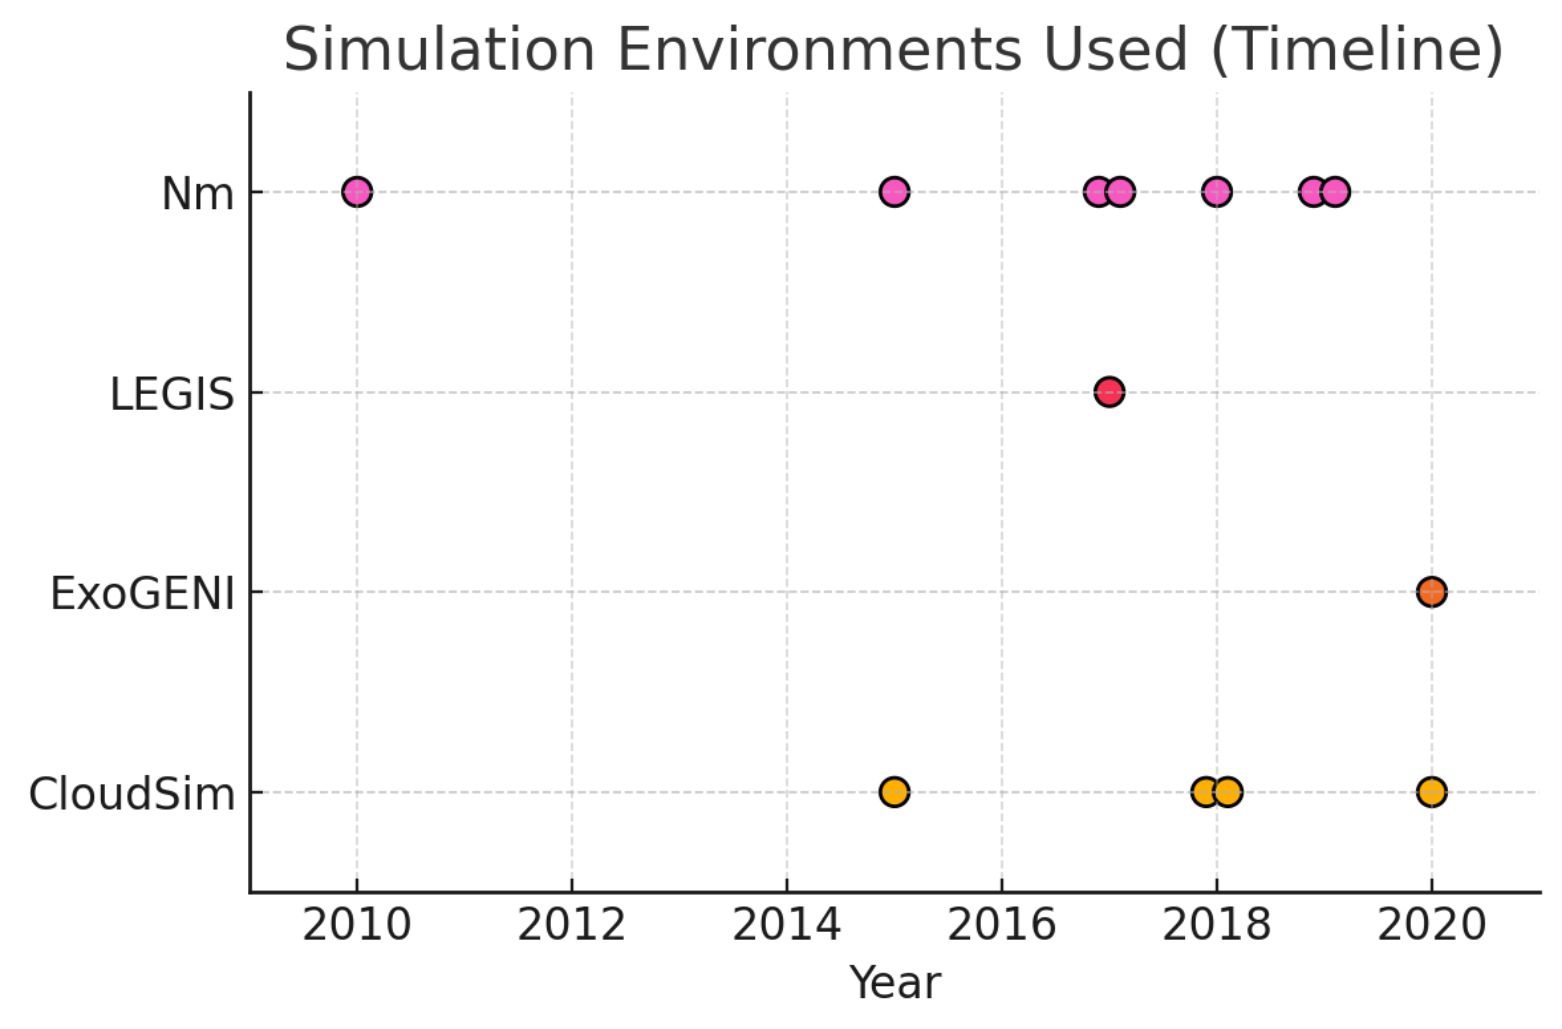
\includegraphics[width=0.9\columnwidth]{sections/Timeline.png}
    \caption{Timeline of simulation environments used in each paper (2010--2020). }
    \label{fig:timeline}
\end{figure}

Additionally, we plotted the relationship between the number of CPU cores and the \textit{energy delta} (the difference $P_{\max} - P_{\textit{idle}}$), shown in Figure~\ref{fig:energy_delta}. This second figure highlights how dynamic power consumption scales with increased core counts and is further distinguished by algorithm type (color) and simulation environment (marker shape).

\end{multicols}
\begin{figure}[H]
    \centering
    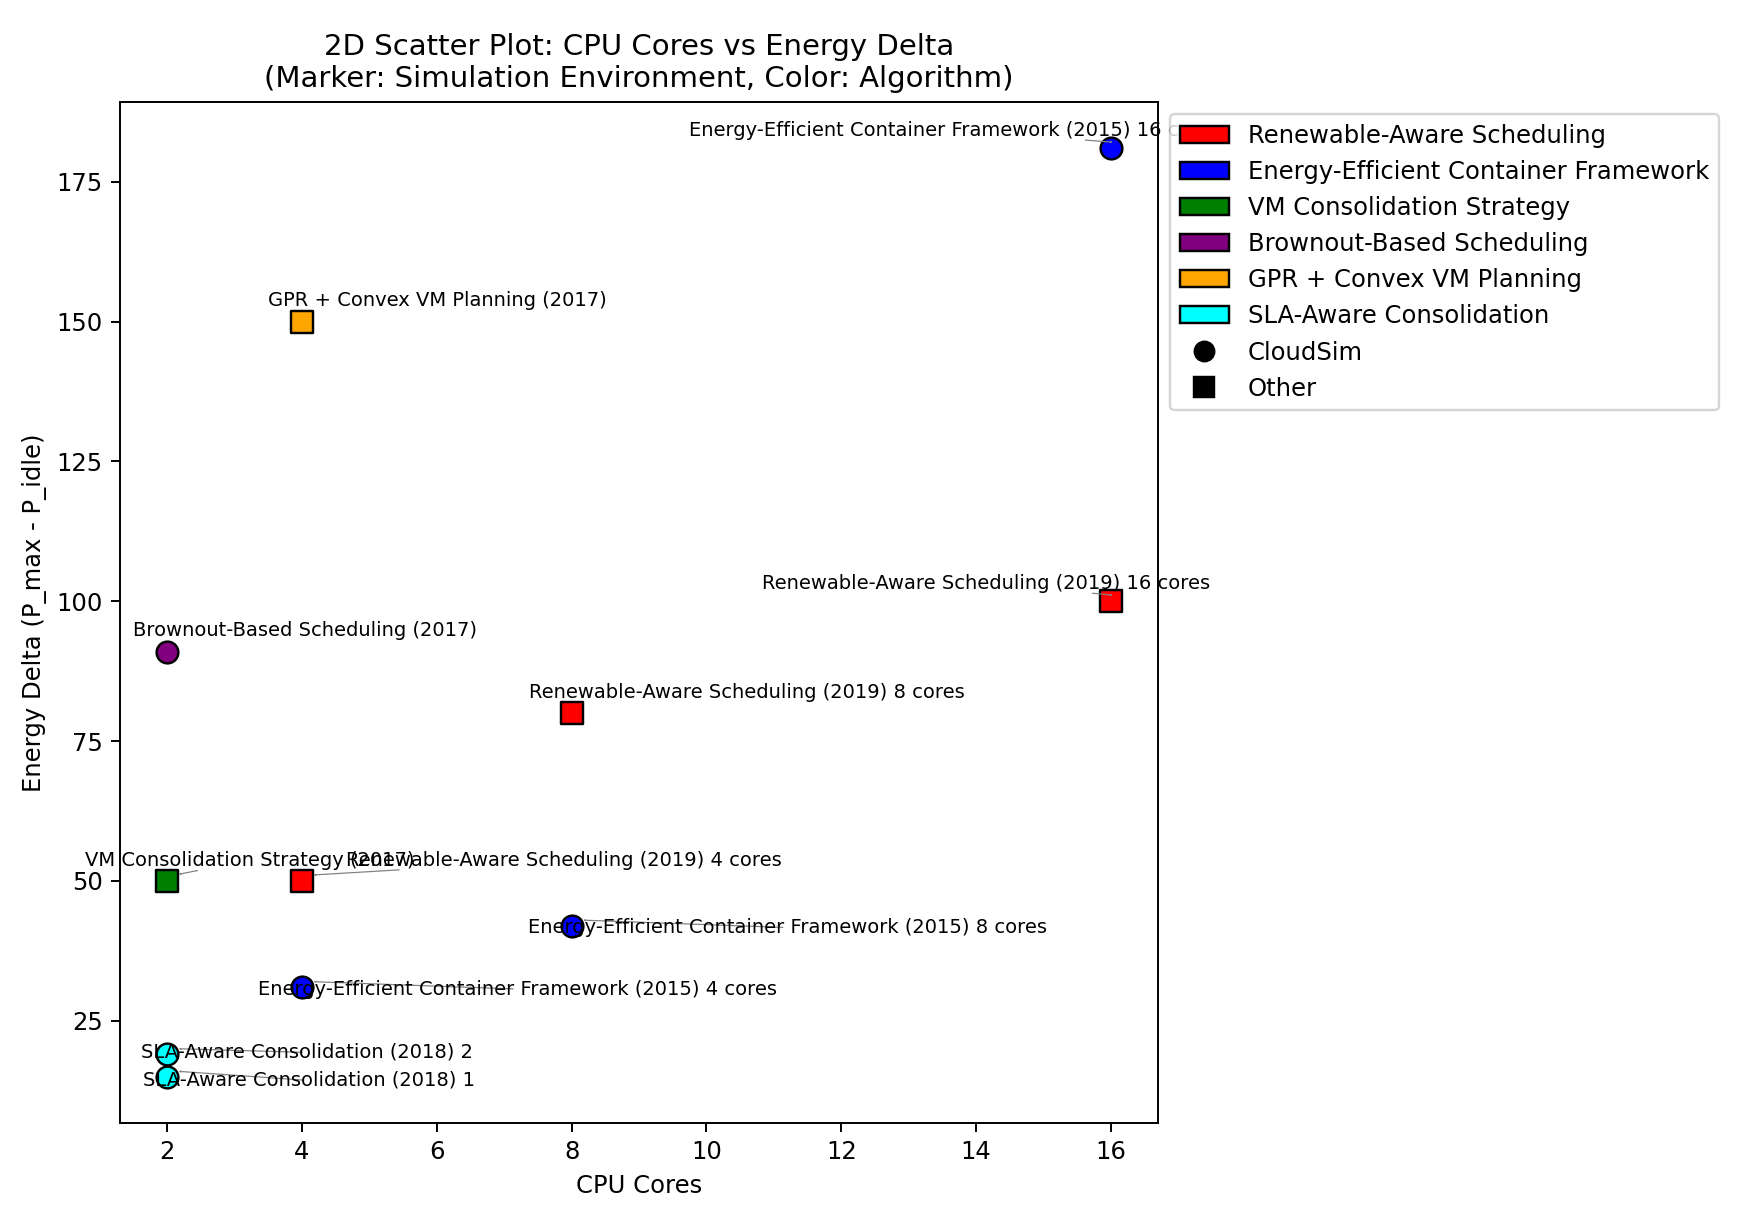
\includegraphics[width=0.9\columnwidth]{sections/Energy.png}
    \caption{2D Scatter Plot: CPU cores vs. Energy Delta $(P_{\max} - P_{\textit{idle}})$.}
    \label{fig:energy_delta}
\end{figure}
\begin{multicols}{2}

\end{multicols}
